\documentclass{standalone}
\usepackage{tikz}
\usepackage{xcolor}
\usetikzlibrary{patterns, positioning}
\usetikzlibrary{shapes.misc}
\usepackage[outline]{contour}
\contourlength{1.5pt} 


\begin{document}
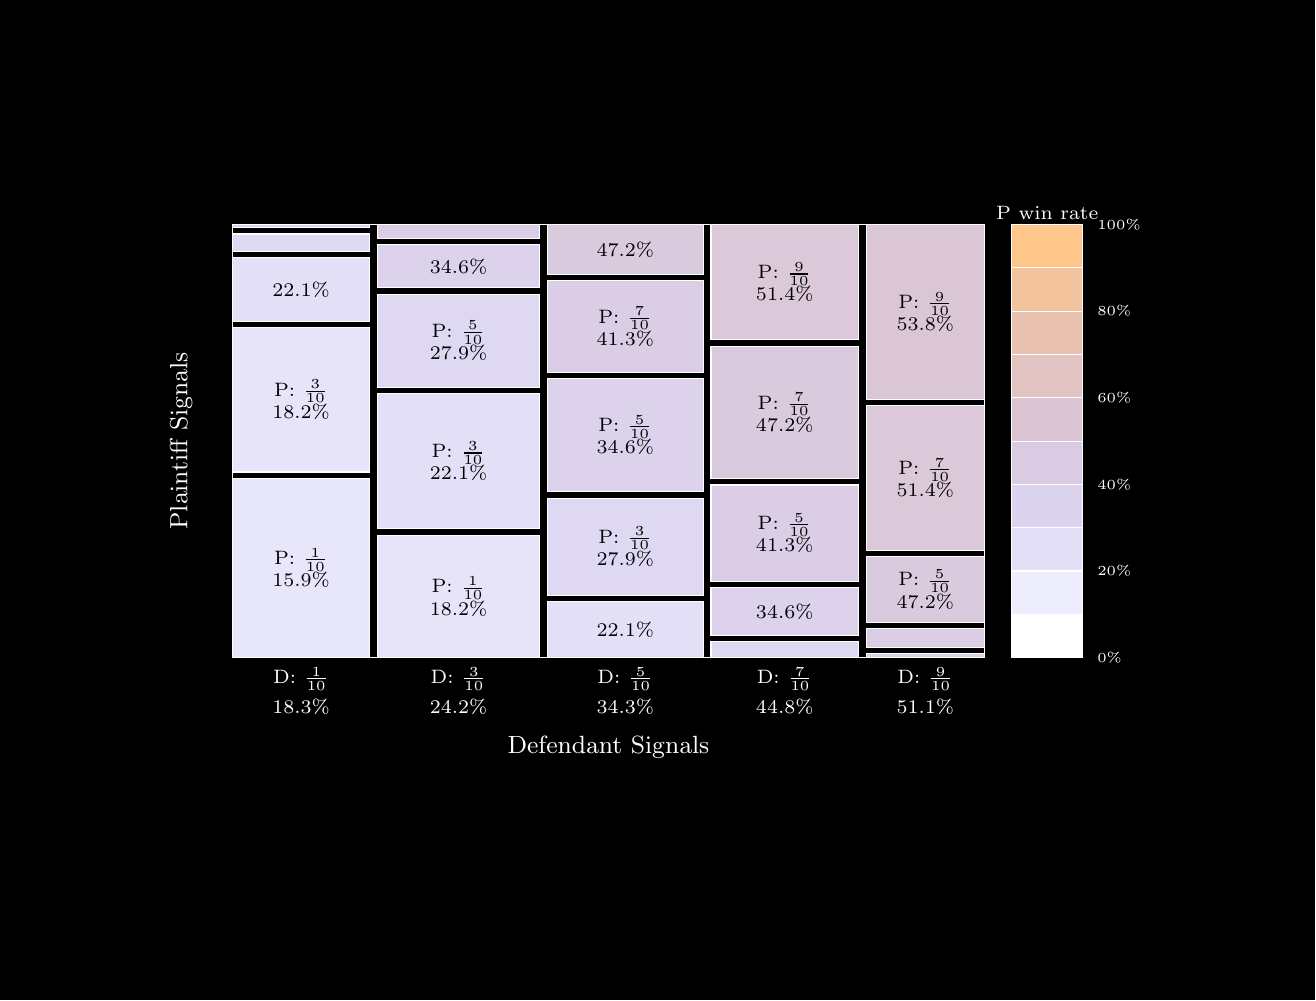
\begin{tikzpicture}
\newcommand{\DFractionOffset}{0.4}
\newcommand{\AxisLabelYAdjust}{-0.235}
\pagecolor{black}
\draw[fill=black, draw=none] (-2,-2) rectangle (14,10);
\draw[draw=white] (0.6,2) rectangle (10.15,7.5);
\draw[fill=blue!84!orange!16!white!66!white, draw=white] (0.6,2) rectangle (2.3438,4.2768);
\draw (1.471895631147195, 3.1383799254939606) node[font=\scriptsize, text=black, align=center] {P: $\frac{1}{10}$\\ 15.9\%};
\draw[fill=blue!82!orange!18!white!65!white, draw=white] (0.6,4.3568) rectangle (2.3438,6.1926);
\draw (1.471895631147195, 5.274655990810261) node[font=\scriptsize, text=black, align=center] {P: $\frac{3}{10}$\\ 18.2\%};
\draw[fill=blue!78!orange!22!white!64!white, draw=white] (0.6,6.2726) rectangle (2.3438,7.079);
\draw (1.471895631147195, 6.675757362997726) node[font=\scriptsize, text=black, align=center] {22.1\%};
\draw[fill=blue!72!orange!28!white!63!white, draw=white] (0.6,7.159) rectangle (2.3438,7.3794);
\draw[fill=blue!65!orange!35!white!61!white, draw=white] (0.6,7.4594) rectangle (2.3438,7.5);
\draw (1.471895631147195, 1.6) node[anchor=north, font=\scriptsize, text=white] {18.3\%};
\draw (1.471895631147195, {1.6 + \DFractionOffset}) node[anchor=north, font=\scriptsize, text=white] {D: $\frac{1}{10}$};
\draw[fill=blue!82!orange!18!white!65!white, draw=white] (2.4438,2) rectangle (4.5028,3.5547);
\draw (3.473316054918882, 2.7773582917977158) node[font=\scriptsize, text=black, align=center] {P: $\frac{1}{10}$\\ 18.2\%};
\draw[fill=blue!78!orange!22!white!64!white, draw=white] (2.4438,3.6347) rectangle (4.5028,5.3518);
\draw (3.473316054918882, 4.493280253586846) node[font=\scriptsize, text=black, align=center] {P: $\frac{3}{10}$\\ 22.1\%};
\draw[fill=blue!72!orange!28!white!63!white, draw=white] (2.4438,5.4318) rectangle (4.5028,6.6147);
\draw (3.473316054918882, 6.023281260206759) node[font=\scriptsize, text=black, align=center] {P: $\frac{5}{10}$\\ 27.9\%};
\draw[fill=blue!65!orange!35!white!61!white, draw=white] (2.4438,6.6947) rectangle (4.5028,7.2444);
\draw (3.473316054918882, 6.969563897184811) node[font=\scriptsize, text=black, align=center] {34.6\%};
\draw[fill=blue!59!orange!41!white!60!white, draw=white] (2.4438,7.3244) rectangle (4.5028,7.5);
\draw (3.473316054918882, 1.6) node[anchor=north, font=\scriptsize, text=white] {24.2\%};
\draw (3.473316054918882, {1.6 + \DFractionOffset}) node[anchor=north, font=\scriptsize, text=white] {D: $\frac{3}{10}$};
\draw[fill=blue!78!orange!22!white!64!white, draw=white] (4.6028,2) rectangle (6.5781,2.7119);
\draw (5.590479186649333, 2.3559530514713303) node[font=\scriptsize, text=black, align=center] {22.1\%};
\draw[fill=blue!72!orange!28!white!63!white, draw=white] (4.6028,2.7919) rectangle (6.5781,4.0249);
\draw (5.590479186649333, 3.408426723126394) node[font=\scriptsize, text=black, align=center] {P: $\frac{3}{10}$\\ 27.9\%};
\draw[fill=blue!65!orange!35!white!61!white, draw=white] (4.6028,4.1049) rectangle (6.5781,5.546);
\draw (5.590479186649333, 4.825479121702286) node[font=\scriptsize, text=black, align=center] {P: $\frac{5}{10}$\\ 34.6\%};
\draw[fill=blue!59!orange!41!white!60!white, draw=white] (4.6028,5.626) rectangle (6.5781,6.7855);
\draw (5.590479186649333, 6.205755953589869) node[font=\scriptsize, text=black, align=center] {P: $\frac{7}{10}$\\ 41.3\%};
\draw[fill=blue!53!orange!47!white!58!white, draw=white] (4.6028,6.8655) rectangle (6.5781,7.5);
\draw (5.590479186649333, 7.182750503542648) node[font=\scriptsize, text=black, align=center] {47.2\%};
\draw (5.590479186649333, 1.6) node[anchor=north, font=\scriptsize, text=white] {34.3\%};
\draw (5.590479186649333, {1.6 + \DFractionOffset}) node[anchor=north, font=\scriptsize, text=white] {D: $\frac{5}{10}$};
\draw[fill=blue!72!orange!28!white!63!white, draw=white] (6.6781,2) rectangle (8.5515,2.2052);
\draw[fill=blue!65!orange!35!white!61!white, draw=white] (6.6781,2.2852) rectangle (8.5515,2.8894);
\draw (7.614811774138377, 2.587314347330243) node[font=\scriptsize, text=black, align=center] {34.6\%};
\draw[fill=blue!59!orange!41!white!60!white, draw=white] (6.6781,2.9694) rectangle (8.5515,4.1919);
\draw (7.614811774138377, 3.5806737429517375) node[font=\scriptsize, text=black, align=center] {P: $\frac{5}{10}$\\ 41.3\%};
\draw[fill=blue!53!orange!47!white!58!white, draw=white] (6.6781,4.2719) rectangle (8.5515,5.9541);
\draw (7.614811774138377, 5.113005298704243) node[font=\scriptsize, text=black, align=center] {P: $\frac{7}{10}$\\ 47.2\%};
\draw[fill=blue!49!orange!51!white!57!white, draw=white] (6.6781,6.0341) rectangle (8.5515,7.5);
\draw (7.614811774138377, 6.767030572225263) node[font=\scriptsize, text=black, align=center] {P: $\frac{9}{10}$\\ 51.4\%};
\draw (7.614811774138377, 1.6) node[anchor=north, font=\scriptsize, text=white] {44.8\%};
\draw (7.614811774138377, {1.6 + \DFractionOffset}) node[anchor=north, font=\scriptsize, text=white] {D: $\frac{7}{10}$};
\draw[fill=blue!65!orange!35!white!61!white, draw=white] (8.6515,2) rectangle (10.15,2.0472);
\draw[fill=blue!59!orange!41!white!60!white, draw=white] (8.6515,2.1272) rectangle (10.15,2.3685);
\draw[fill=blue!53!orange!47!white!58!white, draw=white] (8.6515,2.4485) rectangle (10.15,3.2848);
\draw (9.400753011260731, 2.866658619206883) node[font=\scriptsize, text=black, align=center] {P: $\frac{5}{10}$\\ 47.2\%};
\draw[fill=blue!49!orange!51!white!57!white, draw=white] (8.6515,3.3648) rectangle (10.15,5.1975);
\draw (9.400753011260731, 4.2811931959598315) node[font=\scriptsize, text=black, align=center] {P: $\frac{7}{10}$\\ 51.4\%};
\draw[fill=blue!46!orange!54!white!57!white, draw=white] (8.6515,5.2775) rectangle (10.15,7.5);
\draw (9.400753011260731, 6.388768774549156) node[font=\scriptsize, text=black, align=center] {P: $\frac{9}{10}$\\ 53.8\%};
\draw (9.400753011260731, 1.6) node[anchor=north, font=\scriptsize, text=white] {51.1\%};
\draw (9.400753011260731, {1.6 + \DFractionOffset}) node[anchor=north, font=\scriptsize, text=white] {D: $\frac{9}{10}$};
\node[font=\small, text=white] at (5.375, {1.1 + \AxisLabelYAdjust}) {Defendant Signals};
\node[font=\small, text=white, rotate=90] at (-0.050000000000000044, 4.75) {Plaintiff Signals};
\draw[draw=white] (10.5,2) rectangle (11.4,7.5);
\draw (10.95, 7.65) node[font=\scriptsize, text=white] {P win rate};
\draw[fill=blue!100!orange!0!white!70!white, draw=white] (10.5,2) rectangle (11.4,2.55);
\draw[fill=blue!89!orange!11!white!67!white, draw=white] (10.5,2.55) rectangle (11.4,3.1);
\draw[fill=blue!78!orange!22!white!64!white, draw=white] (10.5,3.1) rectangle (11.4,3.65);
\draw[fill=blue!67!orange!33!white!62!white, draw=white] (10.5,3.65) rectangle (11.4,4.2);
\draw[fill=blue!56!orange!44!white!59!white, draw=white] (10.5,4.2) rectangle (11.4,4.75);
\draw[fill=blue!44!orange!56!white!56!white, draw=white] (10.5,4.75) rectangle (11.4,5.3);
\draw[fill=blue!33!orange!67!white!53!white, draw=white] (10.5,5.3) rectangle (11.4,5.85);
\draw[fill=blue!22!orange!78!white!51!white, draw=white] (10.5,5.85) rectangle (11.4,6.4);
\draw[fill=blue!11!orange!89!white!48!white, draw=white] (10.5,6.4) rectangle (11.4,6.95);
\draw[fill=blue!0!orange!100!white!45!white, draw=white] (10.5,6.95) rectangle (11.4,7.5);
\draw (11.46, 2) node[anchor=west, font=\tiny, text=white] {0\%};
\draw (11.46, 3.1) node[anchor=west, font=\tiny, text=white] {20\%};
\draw (11.46, 4.2) node[anchor=west, font=\tiny, text=white] {40\%};
\draw (11.46, 5.3) node[anchor=west, font=\tiny, text=white] {60\%};
\draw (11.46, 6.4) node[anchor=west, font=\tiny, text=white] {80\%};
\draw (11.46, 7.5) node[anchor=west, font=\tiny, text=white] {100\%};


\end{tikzpicture}
\end{document}